
%%%%%%%%%%%%%%%%%%%%%%%%%%%%%%%%%%%%%%%%%%%%%%%%%%%%%
%
%
%  	PROBABILITY MODELS - 
%
%
%%%%%%%%%%%%%%%%%%%%%%%%%%%%%%%%%%%%%%%%%%%%%%%%%%%%%

\begin{slide}
\question

\begin{slidesonly}
	\vspace{3cm}
\end{slidesonly}

\begin{center}
\Huge 
\textcolor{LimeGreen}{Probability Models}
\end{center}

	
\end{slide}



\begin{slide}
\question

\SavedDefinitionRender{IntroProbability}

\SavedDefinitionRender{ConditionalProb}

\end{slide}

\begin{slide}

\SavedDefinitionRender{hazard}

\begin{parts}
	\item Show that $\frac{d\tilde{F}_T}{dt} = - f_T$. 
	\item Find an ODE that relates $\tilde{F}_T$ and $h(t)$ and use it to show that
	\[ \tilde{F}_T(t) = e^{-\int_{-\infty}^t h_T(\tau) ~d\tau} \]

	\item Show that the mean satisfies 
	\[\displaystyle 
		\mu_T = \int_{-\infty}^\infty \tilde{F}_T(t) ~dt.
	\]
\end{parts}
	
\end{slide}


\begin{slide}
\question \label{exponential}

\SavedDefinitionRender{Exponential}

Let us study the \textbf{exponential random variable}: 
\[T \sim {\rm Exp}(\gamma).\]

\begin{parts}
	\item Find an expression for its cdf $F_T(t)$.
	\item Find an expression for its ccdf $\tilde{F}_T(t)$.
	\item Find an expression for its hazard function $h_T(t)$.
	\item What is its mean $\mu_T$?
\end{parts}

\begin{slidesonly}
\vspace{3cm}	
\end{slidesonly}

The hazard function is a constant, so knowing that the random variable is yet to occur, doesn't us give any information.

\SavedDefinitionRender{memoryless}


\begin{parts}
\setcounter{partsitem}{4}
	\item Show that the Exponential is memoryless.
\end{parts}
	
\end{slide}


\begin{solution}
\begin{slide}
\begin{parts}

	\item $\displaystyle F_T(t) 
	 		= \int_{-\infty}^t f_T(\tau)~d\tau
	 		= \int_0^t \gamma e^{-\gamma \tau} ~d\tau
%	 		= - e^{-\gamma \tau} \big|_0^t 
	 		= 1-e^{-\gamma t}$
	 
	 \item $\tilde{F}_T(t) = 1 - F_T(t) = e^{-\gamma t}$.

	 \item $\displaystyle h_T(t) = \frac{f_T(t)}{\tilde{F}_T(t)} = \gamma$.

	 \item $\displaystyle \mu_T 
	 		= \int_{0}^\infty \tau f_T(\tau) ~d\tau
	 		= \int_0^\infty \tilde{F}_T(\tau) ~d\tau 
	 		= -\frac{1}{\gamma} e^{-\gamma \tau} \big|_0^\infty
	 		= \frac{1}{\gamma}$
	 	
	 \item 
	 $\displaystyle \Pr(T>t+s|T>t) = \frac{\Pr(T>t+s)}{\Pr(T>t)} = \frac{e^{-\gamma (t+s)}}{e^{-\gamma t}} = e^{-\gamma s} = \Pr(T>s)$.
	 
	

	
\end{parts}


	
\end{slide}

\end{solution}
	




\begin{slide}
\question

Backblaze is a cloud storage company that uses thousands of hard drives\footnote{They publish data on their hard drives \url{https://www.backblaze.com/b2/hard-drive-test-data.html}.}.\\

The failure rate for a hard drive, also known as hazard rate, is composed of three terms:
\begin{center}
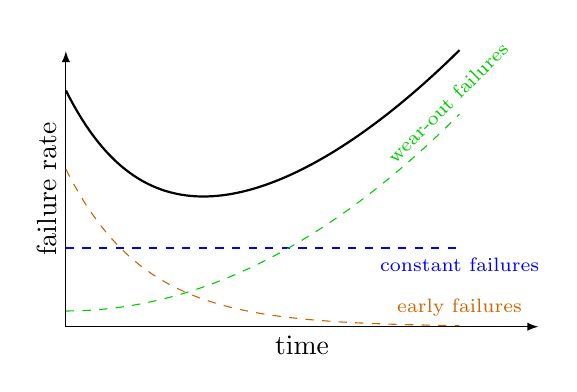
\begin{tikzpicture}
	\draw[latex-latex] (6,0) --node[below] {time} (0,0) --node[above,rotate=90] {failure rate} (0,3.5);
	\draw[dashed,blue] (0,1) -- (5,1) node[below] {\scriptsize constant failures};
   \draw[dashed,orange!80!black,variable=\x,samples=100,domain=0:5] plot({\x},{2*exp(-\x)}) node[above] {\scriptsize early failures}; 
   \draw[dashed,green!80!black,variable=\x,samples=100,domain=0:5] plot({\x},{0.2+\x*\x/10}) node[above,rotate=45] {\scriptsize wear-out failures}; 
   \draw[thick,variable=\x,samples=100,domain=0:5] plot({\x},{1+\x*\x/10+2*exp(-\x)}); 
\end{tikzpicture}
\end{center}

When we add the three terms, we get a \textit{bathtub} curve. \\

Should Backblaze always use the hard drives with the longest mean time between failures (MTBF)?

\begin{parts}
\item Suppose that there are $N$ hard drive types, each with a known fixed cost $c_n$, a known profit $p_n$ per unit time that hard drive is operational, and a random lifetime $T_n$ with a known distribution. Backblaze has limited storage, so they can only have $M$ hard drives. If they use $x_n$ drives of type $n$, what is their profit function?

%$$
%P = \sum_{n=1}^N \left[p_n \sum_{m=1}^{x_n} T_n(m)  - x_n c_n \right]
%$$

\item What is their expected profit?
%$$
%\sum_{n=1}^N \left[x_n p_n \mu_{T_n}  - x_n c_n \right]
%$$

\item If they choose to maximize the expected profit, what is the solution?
\end{parts}

	
\end{slide}


\begin{solution}
\begin{slide}
\begin{parts}
\item The profit function is
\[
P = \sum_{n=1}^N \left[p_n \sum_{m=1}^{x_n} T_n(m) - c_n x_n\right].
\]
and it should be constrained to $\sum_{n=1}^N x_n = M$.

\item Their expected profit is
\[
E(P) = \sum_{n=1}^N (p_n \mu_{T_n} - c_n )x_n.
\]
	
\item We need to find the type of drive $n^\star$ that maximizes
\[ \max_n (p_n \mu_{T_n} - c_n) \]
and buy $M$ hard drives of type $n^\star$ to get an expected profit of 
\[ 
E(P) = M (p_{n^\star} \mu_{T_{n^\star}} - c_{n^\star})
\]
\end{parts}
	
\end{slide}
	
\end{solution}



\begin{slide}

This means that they will \textit{put all their eggs in one basket}!

This is a risky strategy. Especially if hard drives with long-lives have a large variance in those lives.

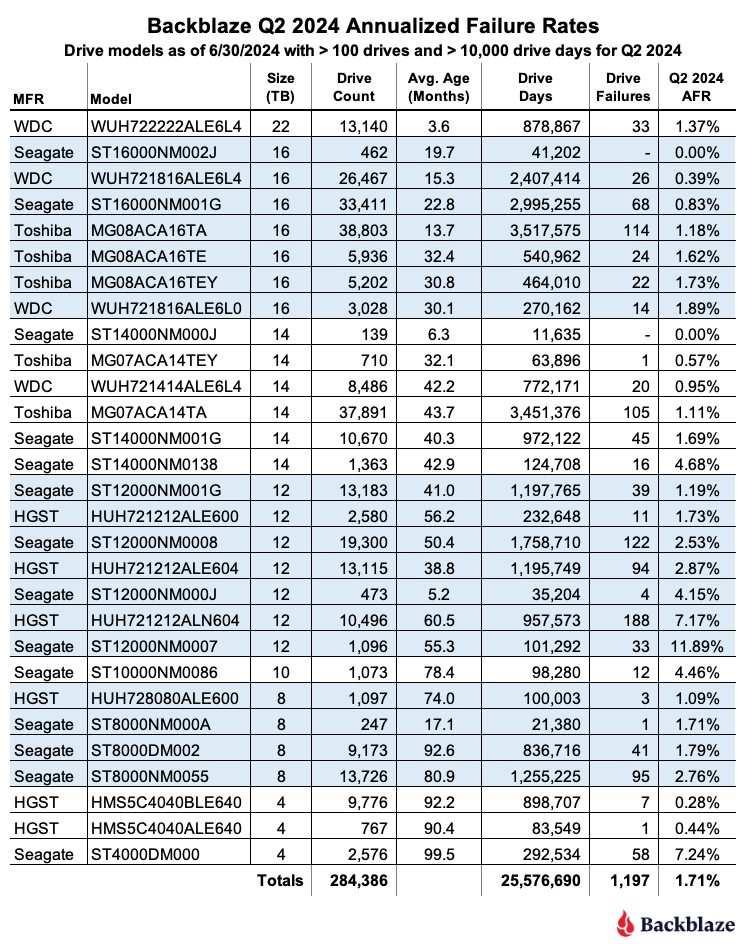
\includegraphics[width=150pt]{images/backblaze-hdd.png}

To account for this, we can add a constraint that the variance of the profit $\sigma_P^2$ not be too large.
This will result in a more diverse selection of hard drives.
Unfortunately, for most hard drive lifetime distributions, this constraint is non-linear in the decision variables. 

	
\end{slide}






\begin{slide}
\question \label{ex-poisson}

\SavedDefinitionRender{Poisson}

Start with $N(0) = 0$ and define $p_n(t) = \Pr\big( N(t)=n \big)$, the probability that $n$ events have occurred up to time $t$.


\begin{slidesonly}
	\bigskip
\end{slidesonly}

\begin{parts}
	\item What is $p_n(0)$?
	\item Take $n=0$. Explain in words why $p_0(t) = \tilde{F}_T(t)$.

	\item A different approach:
	\[ 
		\underbrace{\frac{d p_0}{dt}(t)}_{\substack{\text{change in prob}\\\text{that $N(t)=0$}}}
		 = +\underbrace{0}_{\text{can never increase}}
		 -\underbrace{p_{0}(t) h_T(t)}_{\substack{\text{decreases if $N$ was $0$}\\\text{and an event occurs}}}
	\]

	Solve this differential equation to find $p_0(t)$.

	\item For $n>0$, we can find an ODE in a similar way. The change in probability that $N(t)=n$:
	\begin{enumerate}
		\item decreases if ...
		\item increases if ...
	\end{enumerate}
	
	\item Obtain an ODE and show that $p_n(t) = \frac{(\gamma t)^n}{n!} e^{-\gamma t}$ is a solution.
	
	\item Show that it is normalized, i.e. $\displaystyle\sum_{n=0}^\infty p_n(t) = 1$.

	\item Calculate its mean $\displaystyle\sum_{n=0}^\infty n p_n(t)$.
	
	
\end{parts}

	
\end{slide}


\begin{solution}
	

\begin{slide}
\begin{parts}
	\item $p_n(0) = \delta_{n,0}$
	\item It is the probability that no events have occurred until time $t$, which is the complement of the probability of an event happening between time $0$ and $t$, so $p_0(t) = 1 - F_T(t) = \tilde{F}_T(t) = e^{-\gamma t}$.

	\item The ODE is $\frac{d p_0}{dt} = -\gamma p_0$, so the solution is $p_0(t) = e^{-\gamma t}$.

	\item 
	\begin{enumerate}
		\item decreases if $N$ was $n$ and an event occurs imminently
		\item increases if $N$ was $n-1$ and an event occurs imminently
	\end{enumerate}
	
	\item 	
	\[ 
		\underbrace{\frac{d p_n}{dt}(t)}_{\substack{\text{change in prob}\\\text{that $N(t)=n$}}}
		 = +\underbrace{p_{n-1}(t) h_T(t)}_{\substack{\text{increases if $N$ was $n-1$}\\\text{and an event occurs}}}
		 -\underbrace{p_{n}(t) h_T(t)}_{\substack{\text{decreases if $N$ was $n$}\\\text{and an event occurs}}}
	\]
	This gives 
	\[ 
		\frac{dp_n}{dt}(t) = \gamma p_{n-1}(t) - \gamma p_n(t)
	\]
	
	\item The series 
	\[ \sum_{n=0}^\infty \frac{(\gamma t)^n}{n!}  \]
	is the Taylor series for $e^{\gamma t}$.
	
	\item Consider $g_n(t) = \frac{(\gamma t)^n}{n!}$. Then
%	\[
%	g_n'(t) = n \frac{(\gamma t)^{n-1}}{n!}
%	\]
%	and
	\[t g_n'(t) = n g_n(t)\]
	So
	\[ \sum_n n \frac{(\gamma t)^n}{n!} 
		= t \left( \sum_n \frac{(\gamma t)^n}{n!}\right)'
		= t \left( e^{\gamma t} \right)'
		= t \gamma e^{\gamma t} \]
	Thus the mean is $E(N(t)) = \gamma t$, which is typically denoted by $\lambda$.

\end{parts}
	
\end{slide}
\end{solution}


\begin{slide}

\SavedDefinitionRender{Poisson2}
	
\end{slide}



\begin{slide}
\question \label{aquarium}
\begin{problem}[Aquarium Problem\footnote{based on a problem from Meerschaert's `Mathematical Modeling'.}]

A pet store sells large aquariums. They sell approximately \textbf{one aquarium per week} (call this the parameter $\lambda$).

Not wanting to maintain too much stock (the aquariums are large and fragile), the store orders 3 aquariums at the end of the week if they are completely out of stock.

How missed sales result from this policy?
\end{problem}

Let
\begin{itemize}
	\item $X_n = $ number of aquariums in stock at the beginning of week $n$
	\item $D_n=$ number of aquariums demanded in week $n$
\end{itemize}
Any available aquariums that are demanded are purchased and assume that when the store orders aquariums, they arrive right away.


\begin{parts}
	\item Why is $X_n$ random?
	\item Assume that $D_n$ is Poisson distributed. Why is this reasonable?
	\item Then what is $\Pr (D_n = k)$?
	\item There are only 3 states of $D_n$: 1, 2, 3. 
	
	The following diagram shows the possible changes in stock from one week to the next.
	
	Complete the following diagram with the probability of transitioning from one state to another for all the arrows except the ones marked with $\star$.
	
	\begin{center}
	\begin{tikzpicture}[font=\sffamily,scale=0.4]
	 
        % Setup the style for the states
        \tikzset{node style/.style={state, 
                                    minimum width=1cm,
                                    line width=0.3mm,
                                    fill=gray!20!white}}
 
        % Draw the states
        \node[node style] at (0, 0)     (x1)    {$X_n=1$};
        \node[node style] at (6, 0)     (x2)    {$X_n=2$};
        \node[node style] at (3, -5.196) (x3) 	{$X_n=3$};
 
        % Connect the states with arrows
        \draw[every loop,
              auto=right,
              line width=0.3mm,
              >=latex,
              draw=black,
              fill=black]
            (x1) edge[loop above]             node {} (x1)
            (x2) edge[loop above]             node {} (x2)
            (x3) edge[loop below]             node {$\star$} (x3)            
            (x1)     edge[bend right=20]            node {} (x2)
            (x2)     edge[bend right=20]            node {} (x1)
            (x1)     edge[bend right=20]            node {$\star$} (x3)
            (x3)     edge[bend left=20]            node {} (x2)
            (x2)     edge[bend left=20, auto=left] node {$\star$} (x3)
            (x3) edge[bend right=20, auto=right] node {} (x1);
    \end{tikzpicture}
	\end{center} 

	\item For the remaining arrows, marked with $\star$, observe that if there is one aquarium in inventory and 3 clients come, then the store will only be able to sell one of them and order new aquariums, so at the beginning of next week there will be 3 aquariums. Because of this, complete the  remaining $\star$ arrows by using the complementary probability. 

\end{parts}


\end{slide}


\begin{slide}

\begin{parts}
\setcounter{partsitem}{5}
	\item Create a transition matrix $\mathcal{P}$ with
	\begin{itemize}
		\item $P_{ij} = $ probability of transitioning from state $i$ to $j$
	\end{itemize}
	
	\item Let 
	\[ 
	\vec{\pi}_n = \mat{ 	\Pr(X_n = 1) \\
					\Pr(X_n = 2) \\
					\Pr(X_n = 3) }
	\]
	Find a relation between $\vec{\pi}_{n+1}$ and $\vec{\pi}_n$.
	
	\item Use \href{https://utoronto.syzygy.ca/jupyter/user-redirect/git-pull?repo=https://github.com/bigfatbernie/IBLMathModeling&subPath=book/python/aquarium.ipynb}{\tt aquarium.ipynb} to approximate the solution for the long term states. 
		Interpret the results.

	\item The original question was about how much business is the store missing. Write the expected percentage of weeks when the store lost at least one sale as a probability.
	
	\item Calculate $W$:
	\begin{align*}
	W 	& = \lim_{n \to \infty} \Pr(D_n > X_n) \\
		& = \lim_{n \to \infty} \sum_{i=1}^3 \Pr(D_n>X_n | X_n = i) \Pr (X_n = i),
	\end{align*}
	using the limiting vector $\vec{\pi}$ found. Interpret the result.
	
	\item We can calculate the average lost sales too by considering:
	\[
	L	= \lim_{n \to \infty} \sum_{i=1}^3 (D_n - i) \Pr(D_n>X_n | X_n = i) \Pr (X_n = i).
	\]
	
	Calculate $L$, the expected number of lost aquarium sales. Interpret the results.
	
	\item What is $S(L^\star, \lambda)$?
\end{parts}

	
\end{slide}




\begin{solution}
\begin{slide}
\begin{parts}
	\item Because $D_n$ is random.  
	\item Because the arrival of customers can happen at any time, they are independent of each other, and they don't depend on $t$ (in reality they do), but because we are measuring in weeks, it's ok.
	\item $\Pr(D_n=k) = \frac{\lambda^k}{k!} e^{-\lambda}$.
	\item 
	
	\begin{center}
	\begin{tikzpicture}[font=\sffamily,scale=0.5]
	 
        % Setup the style for the states
        \tikzset{node style/.style={state, 
                                    minimum width=1cm,
                                    line width=0.3mm,
                                    draw=black,
                                    fill=gray!20!white}}
 
        % Draw the states
        \node[node style] at (0, 0)     (x1)    {\textcolor{black}{$X_n=1$}};
        \node[node style] at (6, 0)     (x2)    {\textcolor{black}{$X_n=2$}};
        \node[node style] at (3, -5.196) (x3) 	{\textcolor{black}{$X_n=3$}};
 
        % Connect the states with arrows
        \draw[every loop,
              auto=right,
              line width=0.3mm,
              >=latex,
              draw=black,
              fill=black]
            (x1) edge[loop above]             node {$e^{-\lambda}$} (x1)
            (x2) edge[loop above]             node {$e^{-\lambda}$} (x2)
            (x3) edge[loop below]             node {$1-\lambda e^{-\lambda}-\frac{\lambda^2}{2}e^{-\lambda}$} (x3)            
            (x2)     edge[bend right=20]            node {$\lambda e^{-\lambda}$} (x1)
            (x1)     edge[bend right=20]            node {$1-e^{-\lambda}$} (x3)
            (x3)     edge[bend left=20]            node {$\lambda e^{-\lambda}$} (x2)
            (x2)     edge[bend left=20, auto=left] node {$1-e^{-\lambda}-\lambda e^{-\lambda}$} (x3)
            (x3) edge[bend right=20, auto=right] node {$\frac{\lambda^2}{2}e^{-\lambda}$} (x1);
    \end{tikzpicture}
	\end{center} 
	
%\setcounter{partsitem}{5}	
%
%	\item \[ 
%			\mathcal{P} 
%				= \mat{ 	e^{-\lambda} & 0 & 1 - e^{-\lambda} \\
%						\lambda e^{-\lambda} & e^{-\lambda} & 1 - e^{-\lambda} - \lambda e^{-\lambda} \\
%						\frac{\lambda^2}{2} e^{-\lambda} & \lambda e^{-\lambda} & 1 - \lambda e^{-\lambda} - \frac{\lambda^2}{2}e^{-\lambda} }
%			\]
%
\end{parts}
	
\end{slide}

\begin{slide}
\begin{parts}
\setcounter{partsitem}{5}	

	\item \[ 
			\mathcal{P} 
				= \mat{ 	e^{-\lambda} & 0 & 1 - e^{-\lambda} \\
						\lambda e^{-\lambda} & e^{-\lambda} & 1 - e^{-\lambda} - \lambda e^{-\lambda} \\
						\frac{\lambda^2}{2} e^{-\lambda} & \lambda e^{-\lambda} & 1 - \lambda e^{-\lambda} - \frac{\lambda^2}{2}e^{-\lambda} }
			\]

	\item We have $\vec{\pi}_{n+1} = \vec{\pi}_n \mathcal{P} 
		 				\quad \Leftrightarrow \quad \vec{\pi}_{n+1} = \mathcal{P}^T \vec{\pi}_n$.
	\item The long term result is: $\vec{\pi} = \mat{0.28471134 \\0.26313999 \\0.45214867}$.


	This means that with $\lambda =1$, that is with 1 expected customer per week, the store should expect to have :
	\begin{itemize}
		\item 1 aquarium in inventory 28.5\% of the weeks
		\item 2 aquariums in inventory 26.3\% of the weeks
		\item 3 aquariums in inventory 45.2\% of the weeks
	\end{itemize}
	
	This means that about half of the time, they have a full inventory. Perhaps this is due to the fact that they ran out of aquariums and just ordered more, so they might be losing a lot of sales when they run out of stock.
	
	\item It is the probability that the demand is higher than the inventory: $\Pr(D_n > X_n)$. 
	
	\begin{slidesonly}
		\bigskip	
	\end{slidesonly}

	\item $W$ is the long term expected percentage of weeks when sales are lost:\\[-20pt]
	\begin{align*}
		W 	
			& = \lim_{n \to \infty} \sum_{i=1}^3 \Pr(D_n>X_n | X_n = i) \Pr (X_n = i) \\
			& = \lim_{n \to \infty} \sum_{i=1}^3 \Pr (X_n = i) \sum_{j=i+1}^\infty \Pr(D_n=j)\\
			& = \sum_{i=1}^3 \pi_i \sum_{j=i+1}^\infty \frac{\lambda^j}{j!} e^{-\lambda} \\
			& = e^{-\lambda} \left[ \pi_1 \sum_{j=2}^\infty \frac{\lambda^j}{j!} + \pi_2  \sum_{j=3}^\infty \frac{\lambda^j}{j!} + \pi_3  \sum_{j=4}^\infty \frac{\lambda^j}{j!} \right]
	\end{align*}
	The series in $j$ is the tail of the Taylor series for the exponential $e^{\lambda}$, so we can write it as \\[-15pt]
	\begin{align*}
	W = & e^{-\lambda}  \left[ \pi_1 ( e^\lambda - 1 - \lambda ) + \pi_2 ( e^\lambda - 1 - \lambda - {\textstyle \frac{\lambda^2}{2}}) \right.\\ 
		& \left.+ \pi_3 ( e^\lambda - 1 - \lambda - {\textstyle \frac{\lambda^2}{2}- \frac{\lambda^3}{6}}) \right]
	\end{align*}
%	\begin{align*}
%	W = &   \left[ \pi_1 ( 1 - (1 + \lambda)e^{-\lambda} ) + \pi_2 ( 1 - (1 + \lambda + {\textstyle \frac{\lambda^2}{2}})e^{-\lambda}) \right.\\ 
%		& \left.+ \pi_3 (1 - (1 + \lambda + {\textstyle \frac{\lambda^2}{2} + \frac{\lambda^3}{6}})e^{-\lambda}) \right]
%	\end{align*}


	Using \href{https://utoronto.syzygy.ca/jupyter/user-redirect/git-pull?repo=https://github.com/bigfatbernie/IBLMathModeling&subPath=book/python/aquarium-sol.ipynb}{\tt aquarium-sol.ipynb}, we get $W = 0.105$, which means that the store loses sales about 11\% of the weeks.
	
\end{parts}


\end{slide}


\begin{slide}
\begin{parts}
\setcounter{partsitem}{10}
	\item Similarly, we can calculate $L =  0.14256$, so the store should expect to lose an average of 0.14 sales per week. 
	Given that the expected number of sales is 1 per week, this is about 14\% of their business and it might be worthwhile to re-evaluate their stocking policy. 
	
	\item To calculate the sensitivity, we need the approximate formula:
	\[
	S(L,\lambda) \approx \frac{L(1+\Delta)-L(1)}{\Delta} \cdot \frac{1}{L(1)} = 1.859
	\]
	
	Which is just moderately sensitive to $\lambda$.

\end{parts}

\rule{\textwidth}{0.4pt}

I also calculated the expected number of sales (should be less than $\lambda$ since we are losing some sales):
\begin{align*}
E % & = \sum_{i=1}^3 \sum_{j=1}^\infty P(D_n=j) P(X_n=i) S_{ij}\\
	& = \sum_{i=1}^3 \sum_{j=1}^i j P(D_n=j) P(X_n=i) + \sum_{i=1}^3 \sum_{j=i+1}^\infty i P(D_n=j) P(X_n=i)\\
 & = \sum_{i=1}^3 \sum_{j=1}^i j \frac{\lambda^j}{j!} e^{-\lambda}\pi_i + \sum_{i=1}^3 \sum_{j=i+1}^\infty i \frac{\lambda^j}{j!} e^{-\lambda} \pi_i \\
 & = e^{-\lambda} \left[\sum_{i=1}^3 \pi_i \lambda \sum_{j=0}^{i-1} \frac{\lambda^j}{j!} \pi_i + \sum_{i=1}^3 i \pi_i \sum_{j=i+1}^\infty i \frac{\lambda^j}{j!} \right] \\ 
 & = 0.857 \quad \text{ for }\lambda=1.
\end{align*}
So the store only makes about 85.7\% of possible sales.

\rule{\textwidth}{0.4pt}

I ran the code for values of $\lambda \in (0,10]$ to get the plots:

\begin{center}
	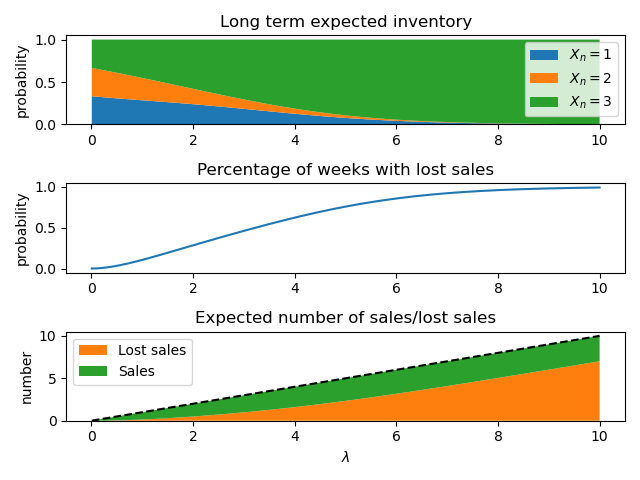
\includegraphics[width=200pt]{images/aquarium.png}
\end{center}

Observe how the number of sales converges to $3$ as $\lambda \to \infty$, which makes sense since that is the maximum inventory. The more clients that come to the store, the more likely to sell all the inventory every week.


	
\end{slide}

\end{solution}



\begin{slide}
\question

Construct a Markov chain model for the heat equation interpreting it as particles randomly bumping around and averaging their temperature when they meet.

	
\end{slide}




\begin{slide}
\question
\begin{problem}[Stochastic Simulation]
It is very rare to be able to obtain analytic results for probabilistic models, so we will study simulating them.
\end{problem}

\SavedDefinitionRender{discrete-event}

\SavedDefinitionRender{tau-leaping}

Here is some code simulating an Exponential Distribution using each method.
\begin{itemize}
	\item \href{https://utoronto.syzygy.ca/jupyter/user-redirect/git-pull?repo=https://github.com/bigfatbernie/IBLMathModeling&subPath=book/python/numerical-stochastic.ipynb}{\tt numerical-stochastic.ipynb}
\end{itemize}

	
\end{slide}



\begin{slide}
\question \label{aquarium2}

Recall Exercise \ref{aquarium}. 

\begin{parts}
	\item Using the Jupyter Notebook 	\href{https://utoronto.syzygy.ca/jupyter/user-redirect/git-pull?repo=https://github.com/bigfatbernie/IBLMathModeling&subPath=book/python/aquarium-part2.ipynb}{\tt aquarium-MonteCarlo.ipynb}, simulate the aquarium problem.

	\item The store is considering an alternative re-stocking policy: when the stock is down to 1 aquarium, they flip a coin and decide whether to re-stock to 3 aquariums or not.
	
	Simulate this new store policy in the same Jupyter Notebook and compare the results.
	
	\item Run the last part of the Jupyter Notebook to combine the results of these two policies. You need to add titles and legends to the graphs, and labels to the $x-$ and $y-$ axes. Compare the results.

	\item \label{aquarium2:economic} Create an economic model for the store that includes: profit from each aquarium sale, stocking cost per aquarium in stock, shipping cost when re-ordering new aquariums.
	
		Evaluate which of the previous two policies is better. 
\end{parts}

\end{slide}


\begin{solution}
\begin{slide}
Solution python: \href{https://utoronto.syzygy.ca/jupyter/user-redirect/git-pull?repo=https://github.com/bigfatbernie/IBLMathModeling&subPath=book/python/aquarium-MonteCarlo-sol.ipynb}{\tt aquarium-MonteCarlo-sol.ipynb}

\begin{parts}	
	\item Plot one simulation for the original re-stocking policy.
	
		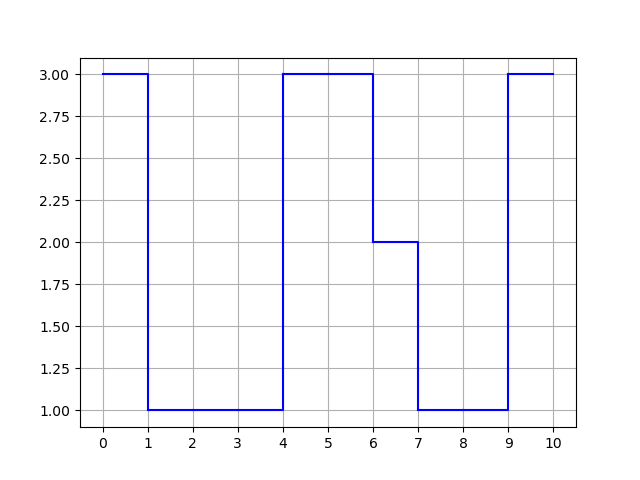
\includegraphics[width=0.4\textwidth]{images/aquarium-sim-og.png}
	\item Plot the same simulation for the modified re-stocking policy.
	
		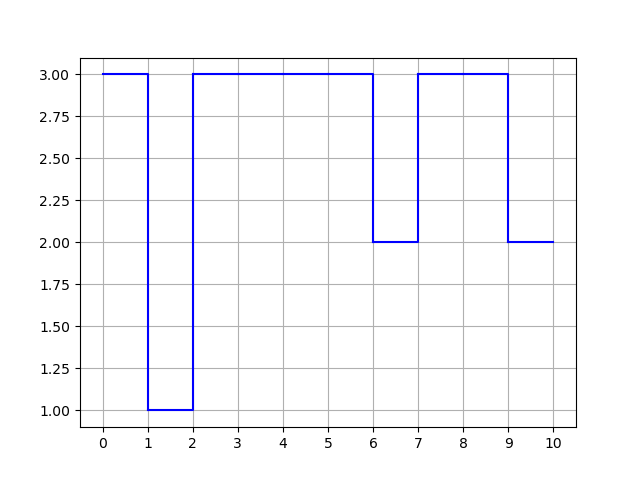
\includegraphics[width=0.4\textwidth]{images/aquarium-sim-mod.png}
		
		
	Observations:
	\begin{itemize}
		\item Week 1: the modified store decided not to order new aquariums, even though they only had 1 in stock
		\item Week 2: the modified store re-stocked
		\item Week 3: the original store had 1 aquarium in stock and sold it, then re-stocked
		\item Week 3: the modified store, had 3 aquariums in stock and sold at least 2, because they also re-stocked
		\item Week 3: This means that the original store lost 1 or 2 more sales than the modified store.
	\end{itemize}	
	
	
	\item From the plots below, we can see that the modified store loses much fewer sales.
\end{parts}	

		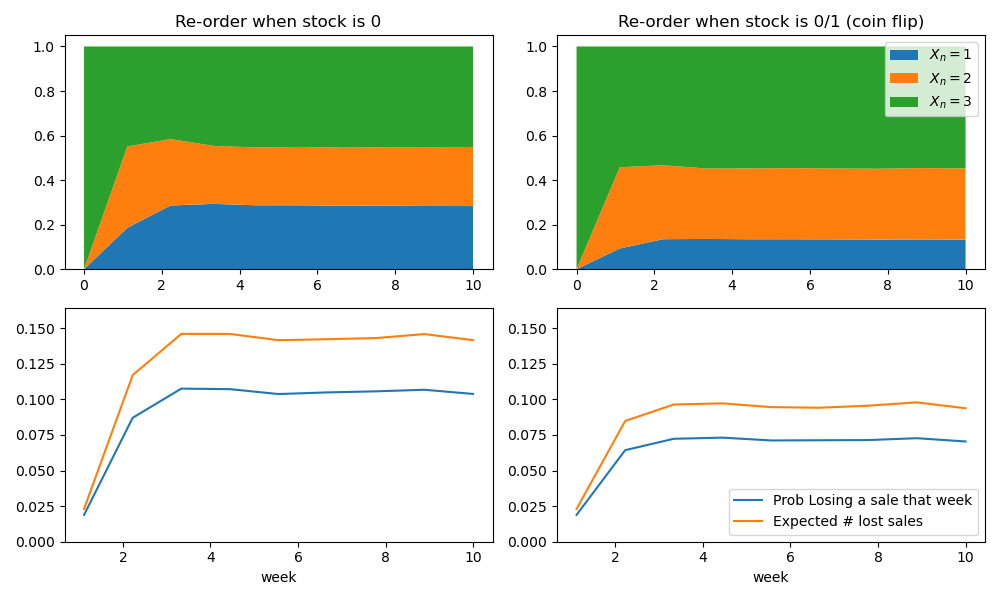
\includegraphics[width=0.75\textwidth]{images/aquarium-sim.png}
	

\end{slide}
	
\end{solution}



\begin{slide}
\question \label{SIR_stochastic}
	
Recall the SIR model:
\begin{align*}
\frac{dS}{dt} 	& = - \beta SI \\
\frac{dI}{dt} & = \beta SI - \gamma I \\
\frac{dR}{dt} & = \gamma I
\end{align*}

We now want to create a stochastic simulation for the same model:
\begin{itemize}
	\item A \textit{susceptible} individual becomes \textit{infected} with probability $\beta I$ per unit time;
	\item An \textit{infected} individual becomes \textit{recovered} with probability $\gamma$ per unit time.
\end{itemize}

An \textit{event} happens when one of these two changes of circumstances happens and we assume that the time between events is \textit{memoryless}, hence it should be \textit{exponentially} distributed with the appropriate rate.

Since the number of infected individuals changes with every event, the rate will need to be updated with each event.

\begin{parts}
	\item Explain why the \textit{discrete event} method will give a better approximation than the  \textit{$\tau$-leaping} method.
	\item We are expecting lots of events, so we will use the $\tau$-leaping method.
		we use the binomial distribution (the discrete version of the Poisson distribution) to determine whether an individual became infected or not.
		Then complete the following for \textbf{one time step} of length $\Delta t$:
		\begin{itemize}
			\item $\Pr($new infectives$=k)\quad =\quad $
			\item $\Pr($new recovereds$=k)\quad =\quad $
		\end{itemize}
	\item Create a simulation for $t\in [0,10]$ and $\Delta t = 0.1$ with:
	\begin{itemize}
		\item Initial population: $S_0=99$, $I_0=1$, $R_0=0$
		\item Infection rate: $\beta=0.1$ (which means $R_0=10$)
		\item Recovery rate: $\gamma =1$
	\end{itemize}
	\item Compare the differences with the deterministic continuous model.
\end{parts}

\end{slide}


\begin{solution}
\begin{slide}
\begin{parts}
	\item With the \textit{discrete event} method, we recalculate the rates with every event, but with the \textit{$\tau$-leaping} method, we don't, we calculate how many events happen in a predetermined timestep size. Since in this model, the rate changes with each event, the discrete event method is more accurate.

	\item 

		$\Pr($new infectives$=k)\quad =\quad {{S}\choose{k}} (\Delta t \beta I)^k (1-\Delta t \beta I)^{S-k}$
		
		$\Pr($new recovereds$=k)\quad =\quad {{I}\choose{k}} (\Delta t \gamma)^k (1-\Delta t \gamma)^{I-k}$

		
	\item The first graph is the result of 10 simulations with \href{https://utoronto.syzygy.ca/jupyter/user-redirect/git-pull?repo=https://github.com/bigfatbernie/IBLMathModeling&subPath=book/python/SIR-stochastic-sol.ipynb}{\tt SIR-stochastic-sol.ipynb}
	
	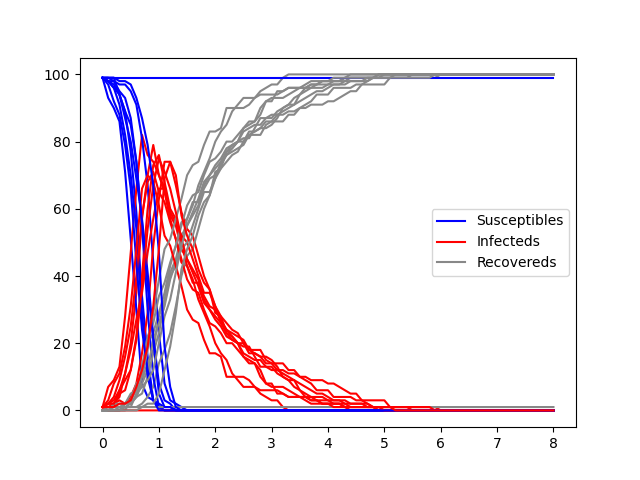
\includegraphics[width=0.5\textwidth]{images/SIR-stochastic1.png}

	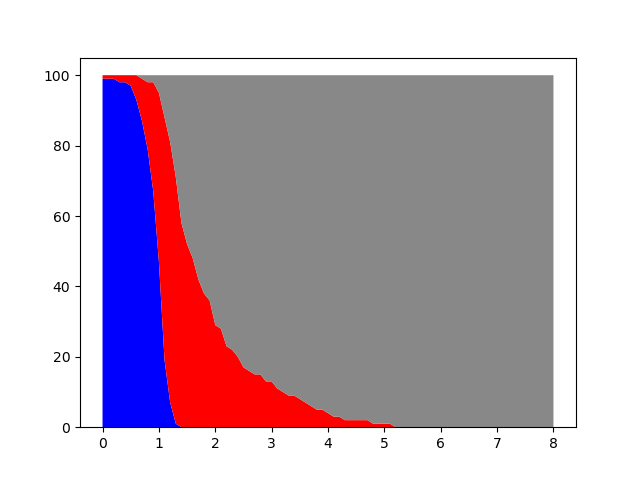
\includegraphics[width=0.5\textwidth]{images/SIR-stochastic2.png}
	
	\item Observe how on one of the simulations, no one else became infected, which would not be possible on the continuous model. Also note that the infected population actually becomes zero in finite time as opposed to asymptotically converging to 0 in the continuous model.
\end{parts}
	
\end{slide}
	
\end{solution}



\begin{slide}
\question

\textbf{Monte Carlo Simulations} and their accuracy.

The simulations we have done with the aquarium and SIR models are called Monte Carlo simulations. These rely on running the simulations again and again, which can take a long time. To compare the accuracy with other numerical methods:

\begin{itemize}
	\item Monte Carlo has square-root convergence: To be 2x more accurate, we need to run it 4x more
	\item Euler has linear convergence: To be $2^1$x more accurate, we need to run it 2x more
	\item Runge-Kutta 4 has 4th order convergence: To be $2^4$x more accurate, we need to run it 2x more
\end{itemize}

They can be very convenient though to run through examples and try different strategies, e.g. for the aquarium store, changing the re-stocking policy required 1-2 different lines of coding.

\end{slide}


\begin{slide}
\question

\begin{problem}[Optimization with Stochastic Simulation]

We want to continue on the idea of Exercise \ref{aquarium2}.\ref{aquarium2:economic}.

We assume the following:
\begin{enumerate}
	\item Each delivery has a cost \$$d$ independent of the number of aquariums shipped.
	\item Each sale has a profit of \$$s$.
	\item Each item in inventory has a small probability $\rho$ of being damaged during the week and that would incur as a cost of \$$c$. The aquariums are damaged independently, so the number of damaged aquariums is binomial $K \sim B(X_n,\rho)$.
\end{enumerate}

We want to optimize the profit.
\end{problem}

\begin{slidesonly}
\vspace{2cm}	
\end{slidesonly}


\begin{parts}
	\item What is the formula for the profit on week $n$ with inventory $X_n$ and demand $D_n$?
	\item Let policy $p(x)$ be the number of aquariums that are reordered when there $x$ aquariums in stock. What are all the possible values $p(x)$? How many possible policies are there?
	\item If the store had a maximum of $m$ aquariums in stock (instead of 3), how many different policies are there?
	\item We can reduce these numbers, because the cost of ordering new aquariums is fixed and doesn't depend on how many aquariums are ordered. 
		
		So if we're willing to re-order to a certain stock $L$ when  the stock is $x$: $p(x) = $?
		then for $y<x$, we should have $p(y)= $?
	
	\item Based on the previous property, how many policies are there for a maximum of $m$ aquariums?
	
\end{parts}

	
\end{slide}



\begin{solution}
\begin{slide}
\begin{parts}
	\item We now have 
	\[
	R_n = \begin{cases}
		s\cdot \min\{D_n,X_n\} - d - c \cdot K_n & \text{if} \min\{D_n,X_n\}>0 \\
		- c \cdot K_n & \text{otherwise}
 	\end{cases}
	\]

	\item $p(3) = 0$, $p(2)\in\{0,1\}$, $p(1)\in\{0,1,2\}$, $p(0)\in\{0,1,2,3\}$, with a total number of possible policies of $4!$.

	\item If the maximum is $m$ aquariums, then there are $(m+1)!$ possible policies, which quickly become too many to check.

	\item So if we're willing to re-order to a certain stock $L$ when  the stock is $x$: $p(x) = L-x$
		then for $y<x$, we should have $p(y)= L-y$?

	\item So we have:
	\[ 
	p(x) = \begin{cases}
			\max\{L-x,0\}	& \text{ if } x < t 	 \\
			0 				& \text{ if } x \geq t 	
		 \end{cases}
	\]
	where $t$ is the level below which the store restocks and $L$ is the level it tries to achieve.

	The possible cases are: $t \in \{1, \ldots, m\}$ and $L \in \{t, \ldots, m\}$, so there are
	\[\sum_{t=1}^m (m-t+1) =\frac12 m(m+1).
	\]
\end{parts}
\end{slide}	
\end{solution}


\begin{slide}
\SavedDefinitionRender{WelfordAlgorithm}


We can now estimate the long term profit by simulating the Markov decision process for each policy.

\begin{itemize}
	\item We can reduce the sampling error by simulating for a large number of weeks (instead of simulating several times).
	\item We can use Welford's algorithm to estimate the mean weekly profit and its variance.
	\item Even though Welford's algorithm reduces the computations needed to calculate the mean and variance, we still need to run the simulation for each possible policy and each week.
\end{itemize}

\begin{parts}
\setcounter{partsitem}{4}
	\item Use Welford's algorithm to calculate all mean and variance of the profit for all the possible policies with $m=3$ (the original setting).
	Use the following values: 
	\begin{itemize}
		\item $\lambda=1$ expected customer per week
		\item Delivery cost $d=\$5$ and sale profit $s=\$20$
		\item Damage probability $\rho=0.01$ and cost $c=\$60$
	\end{itemize}
	
	What is the best policy?
\end{parts}	
	
\end{slide}


\begin{solution}
\begin{slide}
\begin{parts}
\setcounter{partsitem}{4}
	\item Running $1\,000\,000$ weeks and ignoring the first 50 weeks over all 6 policies, we obtain the best policy: 
	\begin{itemize}
		\item \textit{Re-order if the stock $X=0$ or $X=1$.}
		\item The average weekly profit is \$ 15.28
		\item The standard deviation is \$ 20.38
	\end{itemize}
	Below is a graph of the average profits and their standard deviations for each re-stocking policy.
	
	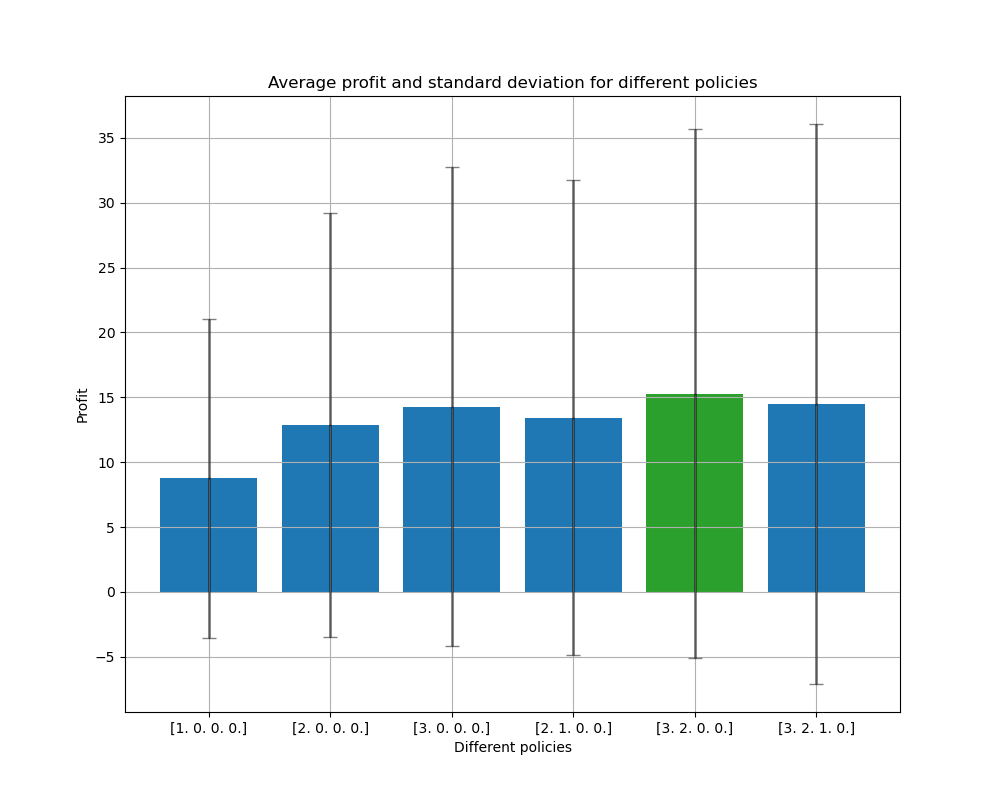
\includegraphics[width=0.5\textwidth]{images/aquarium-policies.png}	

	Code: \href{https://utoronto.syzygy.ca/jupyter/user-redirect/git-pull?repo=https://github.com/bigfatbernie/IBLMathModeling&subPath=book/python/aquarium-MC-policies-sol.ipynb}{\tt aquarium-MC-policies-sol.ipynb}
	
	
\end{parts}


	
\end{slide}	
\end{solution}




\begin{slide}
\question

\SavedDefinitionRender{Q-learning}

\end{slide}

\begin{slide}
Let us now implement the Q-learning algorithm to calculate the optimal policies for different cases.

\begin{parts}
	\item Use \href{https://utoronto.syzygy.ca/jupyter/user-redirect/git-pull?repo=https://github.com/bigfatbernie/IBLMathModeling&subPath=book/python/aquarium-Qlearn.ipynb}{\tt aquarium-Qlearn.ipynb} to calculate the quality of state matrix $Q$ for the original case $m=3$, $\rho=0.01$.
	\item Use this to deduce the best policy in this case.
	\item Use the same process to deduce the optimal policies for the cases $m \in \{1, \ldots 7\}$ and $\rho \in \{0.01, 0.03, 0.05\}$. \\
	
	

	\item Deduce the best policy with an epsilon-greedy Q-learning algorithm: instead of choosing a random action in each iteration, do the following
	\begin{itemize}
		\item Choose the action with best quality with probability $1-\varepsilon$
		\item Choose a random action with probability $\varepsilon$
	\end{itemize}
	\item Deduce the best policy with an epsilon-greedy Q-learning algorithm with a decaying learning rate: the parameter $\varepsilon$ decays to zero as we run more and more iterations.
\end{parts}
\end{slide}



\begin{solution}
\begin{slide}
\begin{parts}
	\item We obtain the matrix
	\[ 
	Q = \mat{
		83.98925114 & 91.15973818 & 95.97324719 & \pmb{99.00385354} \\
		96.15340924 & 96.03440076 & \pmb{98.52386915} &  0. \\
		\pmb{101.72981334} & 98.57852473 &  0.         &  0. \\
		\pmb{104.05899297} &  0.         &  0.         &  0.
	}
	\]
	
	\item To deduce the best policy:
	\begin{itemize}
		\item We need to find the value of $a$ that maximizes the quality for each state
		\item We need to find the maximum for each row and identify the value of that column
	\end{itemize} 
	
	For $m=3$ and $\rho=0.01$, we get:
	\begin{itemize}
		\item 3 \quad 2 \quad 0 \quad 0
	\end{itemize}
	which means that the store should order 3 aquariums when inventory is 0, 2 aquariums when inventory is 1, and not re-stock otherwise.
	
	This matches our previous conclusions.
	
\end{parts}
\end{slide}

\begin{slide}
\begin{parts}
\setcounter{partsitem}{2}
	\item Here are my results:
\end{parts}
	
	\begin{tabular}{|l|l|l|l|}
	\hline
	$\pmb{m}$ & \textbf{policy for $\pmb{\rho=0.01}$}
		& \textbf{policy for $\pmb{\rho=0.03}$}
		& \textbf{policy for $\pmb{\rho=0.05}$} \\ \hline
	\textbf{1} 
		& 1 \quad 0 
		& 1 \quad 0 
		& 1 \quad 0 \\
	\textbf{2} 
		& 2 \quad 1 \quad 0 
		& 2 \quad 0 \quad 0 
		& 2 \quad 0 \quad 0 \\
	\textbf{3} 
		& 3 \quad 2 \quad 0 \quad 0 
		& 3 \quad 2 \quad 0 \quad 0 
		& 2 \quad 0 \quad 0 \quad 0 \\
	\textbf{4} 
		& 4 \quad 3 \quad 0 \quad 0 \quad 0 
		& 3 \quad 2 \quad 0 \quad 0 \quad 0 
		& 2 \quad 0 \quad 0 \quad 0 \quad 0 \\
	\textbf{5}
		& 5 \quad 4 \quad 0 \quad 0 \quad 0 \quad 0 
		& 3 \quad 2 \quad 0 \quad 0 \quad 0 \quad 0 
		& 2 \quad 0 \quad 0 \quad 0 \quad 0 \quad 0 \\
	\textbf{6}
		& 4 \quad 4 \quad 0 \quad 0 \quad 0 \quad 0 \quad 0 
		& 3 \quad 2 \quad 0 \quad 0 \quad 0 \quad 0 \quad 0 
		& 2 \quad 0 \quad 0 \quad 0 \quad 0 \quad 0 \quad 0 \\
	\textbf{7}
		& 5 \quad 4 \quad 0 \quad 0 \quad 0 \quad 0 \quad 0 \quad 0 
		& 3 \quad 2 \quad 0 \quad 0 \quad 0 \quad 0 \quad 0 \quad 0
		& 2 \quad 0 \quad 0 \quad 0 \quad 0 \quad 0 \quad 0 \quad 0\\
	\hline	
	\end{tabular}	

Observe that because the Q-learning algorithm moves randomly from state to state and explores random actions $a$ each iteration, the more possible states and actions, the \textit{weeks} we need and the results are less conclusive.

After running the simulation a few times for $m=6,7$ and $\rho=0.01$, the results varied between these policies:
\begin{itemize}
	\item $4 \quad 4 \quad 0 \quad \cdots$
	\item $5 \quad 4 \quad 0 \quad \cdots$
	\item $6 \quad 4 \quad 0 \quad \cdots$
\end{itemize}

\end{slide}	
\end{solution}




